% !TeX root = ../../main.tex
\section{拆装步骤及操作方式}
\subsection{脉冲器拆装步骤及操作方式}
1）下井前准备

(1) 了解井况，确定套管或者管径规格和深度等基本信息；

(2) 确定工具活动部件是否连接稳固，外观是否存在不合格如裂纹缺口问题，如出现，则不能入井；

(3) 确定工具和其余钻具的连接扣型是否正确；

(4) 可按照推荐排量在井台上检验工具是否能正常振动，喷水口严禁对人。

2）操作方法

(1) 核准下井油管尺寸；

(2) 用“通井规”通井、洗井，若和其他具有通、洗井功能的工具配合使用时可一体化完成；

(3) 将工具缓慢下至设计位置；

(4) 连接管线等地面加压设备后试压；

(5) 开泵加压、冲洗井底，推荐的排量为100L/min-500L/min（直至上返水无污物止）；

(6) 控制出口流量，加大井口压力、排量到设计压力、排量进行正常振动作业；

(7) 每振动1小时，停振10分钟，累计振动作业4-6小时停振、泄压、将工具取出。

3）注意事项

(1) 工具与管柱的连接扣必须拧紧。

(2) 公扣端需要朝下。

(3) 脉冲器在下入过程中如遇阻，应慢慢旋转几圈后再下放。

(4) 不能连续振动超过十分钟。

\subsection{旋转喷头拆装步骤及操作方式}

\subsubsection{拆卸}

准备工具：3mm + 4mm内六方扳手、3/8\inch 套筒、套筒扳手、卸扣工装、可调扳手、链钳\footnote{注：重要！工具需夹紧在装配钳台上。}

\begin{itemize}
	\item 取出筒体2上螺钉
	
	\begin{figure}[htbp]
		\centering
		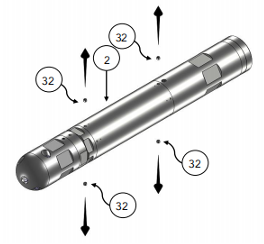
\includegraphics[width=0.5\textwidth]{figure/chapter3/part1-3in1/nozzle-unsetup-step1.png}
		%\caption{拆卸步骤1：取出筒体2上螺钉}
		\label{fig:unscrew_from_body2}
	\end{figure}	
 
		\item 从筒体2上卸掉上接头1和波簧15
\begin{figure}[htbp]
	\centering
	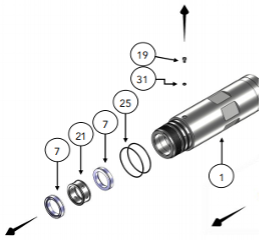
\includegraphics[width=0.5\textwidth]{figure/chapter3/part1-3in1/nozzle-unsetup-step2.png}
	%\caption{拆卸步骤2：卸掉上接头1和波簧15}
	%\label{fig:unscrew_from_body2}
\end{figure}
 
		\item 从上接头1上取出骨架油封7，密封垫环21，卸掉带孔螺钉19取出O型圈31。
\begin{figure}[htbp]
	\centering
	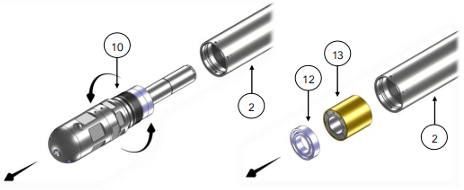
\includegraphics[width=0.7\textwidth]{figure/chapter3/part1-3in1/nozzle-unsetup-step3.png}
	%\caption{拆卸步骤3：取出骨架油封7、密封垫环21与O型圈31}
	%\label{fig:unscrew_from_body2}
\end{figure}
 
		\item 从本体2上卸掉底部帽，取下轴承12和隔套13。
	\begin{figure}[htbp]
		\centering
		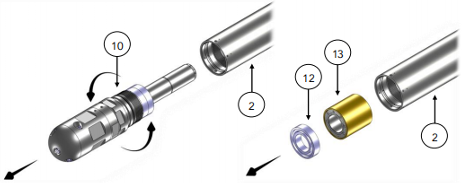
\includegraphics[width=0.7\textwidth]{figure/chapter3/part1-3in1/nozzle-unsetup-step4.png}
		%\caption{拆卸步骤4：卸掉底部帽，取下轴承12和隔套13}
		%\label{fig:unscrew_from_body2}
	\end{figure}
	
	\item 先从旋转头16上卸掉紧定螺钉34，然后将旋转头16从喷头连接体10上卸下来。然后再将紧定螺钉33从喷头连接体10上卸下来，最后将喷头连接体10从芯轴4上卸下来。
	\begin{figure}[htbp]
		\centering
		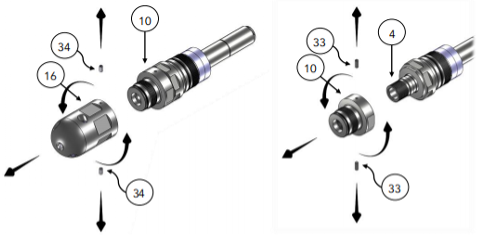
\includegraphics[width=0.7\textwidth]{figure/chapter3/part1-3in1/nozzle-unsetup-step5.png}
		%\caption{拆卸步骤5：卸下旋转头16与喷头连接体10}
		%\label{fig:unscrew_from_body2}
	\end{figure}
	
 
	\item 从芯轴4上卸掉底部帽8和轴承12，插入座3和O型圈26。
	\begin{figure}[htbp]
		\centering
		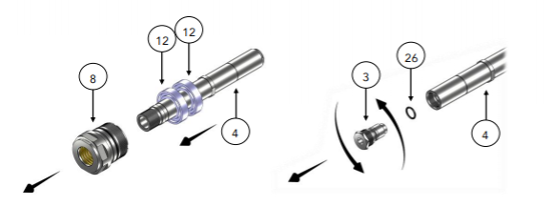
\includegraphics[width=0.7\textwidth]{figure/chapter3/part1-3in1/nozzle-unsetup-step6.png}
		%\caption{拆卸步骤6：卸掉底部帽8和轴承12，取出插入座3与O型圈26}
		%\label{fig:unscrew_from_body2}
	\end{figure}
	
 
	\item 从底部帽8上卸掉平衡活塞座9，取出大弹簧20和O型圈28，取出平衡活塞6。
	\begin{figure}[htbp]
		\centering
		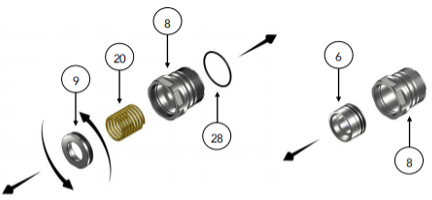
\includegraphics[width=0.7\textwidth]{figure/chapter3/part1-3in1/nozzle-unsetup-step7.png}
		%\caption{拆卸步骤7：卸掉平衡活塞座9，取出大弹簧20、O型圈28与平衡活塞6}
		%\label{fig:unscrew_from_body2}
	\end{figure}
 
	\item 从喷头连接体10上取出O型圈29和30。从平衡活塞上取出骨架油封7和O型圈27。
		\begin{figure}[htbp]
		\centering
		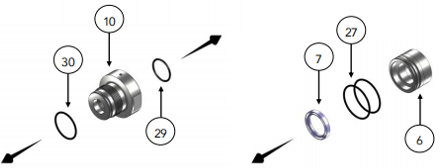
\includegraphics[width=0.7\textwidth]{figure/chapter3/part1-3in1/nozzle-unsetup-step8.png}
		%\caption{拆卸步骤8：取出O型圈29、30与骨架油封7}
		%\label{fig:unscrew_from_body2}
	\end{figure}
 
	\item 从旋转喷头16上取下喷嘴18，从隔套13上取出连通隔套5。
	\begin{figure}[htbp]
		\centering
		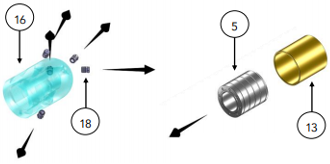
\includegraphics[width=0.7\textwidth]{figure/chapter3/part1-3in1/nozzle-unsetup-step9.png}
		%\caption{拆卸步骤9：取下喷嘴18与连通隔套5}
		%\label{fig:unscrew_from_body2}
	\end{figure}
	
\item 	准备清洗和检测。
	
\end{itemize}
	
\subsubsection{装配}
准备工具：3mm+4mm内六方扳手、3/8\inch 套筒、套筒扳手、扣工装、可调扳手、链钳\footnote{注：重要！工具需夹紧在装配钳台上。}。装配前，检查所有部件是否磨损和腐蚀；润滑所有密封区域并安装O型圈/支撑环。涂抹润滑脂润滑所有螺纹防止粘扣。
\begin{itemize}
	\item 在喷头连接体10上安装O型圈29和O型圈30，在平衡活塞6上安装骨架油封7和O型圈27。
	
	\item 在旋转喷头16上安装喷嘴和引流体17。
	
	\item 在底部帽8上安装O型圈28并依次装入已经小装好的平衡活塞6和大弹簧20和平衡活塞座9。
	
	\item 在芯轴4上安装O型圈26和插入座3，掉头将两件轴承12装入芯轴4并将底部帽8和芯轴连接到位。
	
	\item 将小装好的喷头连接体10和小装好的芯轴4连接到位，并将紧定螺钉33安装在喷头连接体10上。然后将小装好的旋转喷头16和喷头连接体10连接到位后，将紧定螺钉34安装在旋转喷头上。
	
	\item 将底部帽8和筒体2连接到位，在筒体上安装紧定螺钉32，将连通隔套5和隔套13安装，依次将小装后的隔套13、轴承12、波簧15装入筒体2。确保连通隔套5和芯轴4的限位台阶抵紧。
	
	\item 在上接头1上安装O型圈25，O型圈31和带孔螺钉19，并依次在上接头1上装入骨架油封7和密封垫环21。
	
	\item 将装好的上接头1和小装好的筒体2连接到位后安装紧定螺钉32。
	
	\item 安装好之后注油进行旋转测试。
\end{itemize}
	
	
\subsubsection{注油}

准备工具：3mm + 4mm内六方扳手、可调扳手、链钳\footnote{
注（重要）：工具需夹紧在装配钳台上。}

\begin{itemize}

	\item 从筒体2上取掉紧定螺钉32，然后将上接头1从筒体2上卸下来。
	\item 保持旋转喷嘴直立，使用混合硅胶油-1000，直到油位位于筒体2的槽螺孔下方。
 
注：建议让喷嘴直立过夜，使油沉淀。回装喷嘴时，可能需要补注摩擦螺钉下方的油。

	\item 将上接头1和筒体2连接至0.31\inch（7.87 mm），卸掉带孔螺钉19继续上扣至紧扣扭矩。
	
	\item 在筒体2上安装好带孔螺钉19和紧定螺钉32。
 
	\item 安装喷嘴后准备测试。
	\end{itemize}
	
\subsubsection{功能测试}
\begin{itemize}
	
	\item 充油后目视检查工具，检查在修整过程中是否有泄漏或任何密封件损坏。
	
	\item 用手旋转工具，确保其转动平稳，不过度用力，不干涉。
	
	\item 将工具连接到泵上，并开始以最低速率循环通过泵，逐渐增加速率，直到它开始旋转并记录流量。
	
	\item 继续观察恒定流速下是否出现泄漏情况，如果观察到任何泄漏，请参考总装图，以确定哪个密封/密封正在通过。应注意，该工具存在内置的泄漏路径，允许流体通过外壳离开工具。
	
	\item 通常，所有尺寸的工具都会开始以小于0.6次/分的速度旋转，具体值可能存在差异，这取决于芯轴上新唇密封的实际配合状态。如果启动旋转所需的流量高于预期，建议增加流量5$\sim$10 L/min；当新唇密封磨损后，应停止泵送并重复上述操作。
	
	\item 如果不能以所需的流量启动旋转，建议将驱动旋转的两个90度喷嘴更换成更大孔径的喷嘴，以允许喷嘴的流量比例更大。
	\end{itemize}
	
\subsubsection{操作方法}
	\begin{itemize}
		
	\item 该工具可以单独用于清洗油套管，也可以和其他工具组合作业。
	
	\item 将旋转头下入井内距离清洁位置1$\sim$3 m处，开泵循环，排量建议为100 L/min，逐渐加大流量但最大不应超过300 L/min。同时若配置其他工具，需要保持稳定的循环，平稳地上下活动钻具。
	
	\item 起钻时要求平稳、低速、严禁剧烈振动与撞击。
	\end{itemize}

\subsection{液压刮管器拆装步骤及操作方式}

\subsubsection{下井前准备}
		\begin{itemize}
		\item 了解井况，确定套管规格和深度等基本信息；
		\item 根据刮管工艺要求，确定套管是否需要液压启动后再进行刮管。
		\end{itemize}
	
\subsubsection{操作方法}
\begin{itemize}
	\item 下井前按作业要求依次连接好管柱，刮管器前端需接与套管规格对应的扶正器；推荐管柱组合：通井钻头+扶正器+液压刮管器+上部钻柱；
	\item 接上刮管器后，夹紧下接头，用大钳咬住上接头，拧紧刮管器各连接螺纹；
	\item 需要进行刮管作业时，将刮管器下入到所需的井深位置后，投入钢球，开泵进行打压启动作业；其中，刮管器打开压力$=$静液柱压力$+$泵压（绝对压力），即泵压$\ge$绝对压力$-$静液柱压力；
	\item 观察泵压有下降后，说明刮管器启动，此时通过上提、下放工具，如此反复进行刮管作业；
	\item 刮管作业中观察指重表无任何显示，即下放悬重不降、上提悬重不升，表明已刮削干净；
	\item 若上提过程中多次遇阻仍无法上提，可投入复位钢球，开泵将刮刀体强行收回；
	\end{itemize}
\subsubsection{注意事项}
	\begin{itemize}
		\item 工具与管柱的连接扣必须拧紧。
		\item 刮管器在下井过程中如遇阻，应慢慢旋转几圈后再下放。
		\item 刮削过程中，必须始终保持循环畅通。
	\end{itemize}
\subsection{毛刷刮管器拆装步骤及操作方式}
\subsubsection{拆卸}\label{sec:unstep_swiper}
	\begin{itemize}
	\item 去掉防掉螺钉后，用拧扣机拆卸下接头；
	\item 依次取出芯轴上的上扶正套、毛刷体、下扶正套、剪切套、剪切定位套；
	\item 取出所有O型圈与销钉。
	\item 零部件清洗，打磨处理工具表面锈蚀部分；
	\item 清洗并晾干所有零部件。
	\end{itemize}
\subsubsection{装配}
按照\ref{sec:unstep_swiper}所述“拆卸”步骤的反序组装各部件。注意：
\begin{itemize}
	\item 所有密封圈及工具配合面涂润滑油，上扶正套、毛刷体、下扶正套、剪切套、剪切定位套与芯轴间涂抹黄油；
	\item 产品连接螺纹涂钻具螺纹脂；
	\item 上、下接头的上扣扭矩为$10\ \mathrm{kN\cdot m}$；
	\item 产品本体喷涂天蓝色脂肪族面漆，毛刷喷银色漆；
	\item 两端接头螺纹涂防蚀脂并佩戴护丝。
	\end{itemize}
\subsubsection{使用方法}
\begin{itemize}
	\item 	根据井眼尺寸选择合适的套管刮管器。
	\item MSQ型套管刮管器用钻柱送入井底进行刮管作业，情况允许也可以用钢丝绳或者连续油管送入。
\end{itemize}
\subsubsection{操作方法}
\begin{itemize}
	\item 	该工具可以与液压刮管器以及强磁打捞器配合使用，也可以在刮完井之后使用。
	\item 	将MSQ型套管刮管器下到井底离通井位置3$\sim$5 m处，开泵循环。将MSQ型套管刮管器在该位置上下活动，保持循环的情况下平稳地上提钻柱。
	\item 	起钻时要求平稳、低速、严禁剧烈振动与撞击。
\end{itemize}

\section{维护与保养}
\begin{itemize}
	\item 	出井后应清洗干净，并检查各零件。如弹簧失效必须更换。各螺纹涂螺纹脂，各零件涂油，置于阴凉干燥处保存。
\item 	 每次作业后，都应将工具完全拆开并清洗，更换所有O形圈和损坏的弹簧，检查脉冲器上连接螺纹是否有松、退扣的情况发生。用肉眼检查所有密封面和接头丝扣是否损坏，若发现有损坏的零件应予更换，否则会对工具的可靠性产生不利影响。
\item 	在拆卸、保养前，应准备好正确、有效的装配图和工具保养维护说明书及工具维护保养单。
\item 	对高温井的作业和有酸及硫化氢存在的修井作业，应提前更换相应耐腐蚀耐高温密封件和配件。
\end{itemize}

















